\documentclass[conference]{IEEEtran}
\usepackage[spanish,es-nodecimaldot]{babel}
\usepackage{graphicx}
\usepackage{booktabs}
\usepackage{amsmath}
\usepackage{tikz}
\usetikzlibrary{arrows.meta,positioning,fit,backgrounds}
\usepackage{url}
\usepackage{xcolor}

\newcommand{\code}[1]{\texttt{\small #1}}
% Tipograf\'ia: deja que TeX estire espacios antes que invadir el margen, y
% silencia los avisos de l\'inea floja (habituales con tanto identificador).
\emergencystretch=2em
\tolerance=2000
\hbadness=1500

\title{BodyLab: motor antropom\'etrico \emph{local-first} y medici\'on corporal verificable dentro del ecosistema Fitness}

\author{
\IEEEauthorblockN{Alejandro Buend\'ia}
\IEEEauthorblockA{Proyecto Fitness --- BodyLab \& TrainingLab\\
Repositorio: \url{https://github.com/SCP-00/Fitness}\\
Proyecto personal de c\'odigo abierto}
}

\begin{document}
\maketitle

\begin{abstract}
BodyLab es la mitad cient\'ifica del ecosistema Fitness: una aplicaci\'on
\emph{local-first}, sin servidor y sin telemetr\'ia, que registra medidas
antropom\'etricas, las convierte en indicadores matem\'aticos con referencia
expl\'icita, las visualiza en 2D y 3D y educa sobre la ejecuci\'on de ejercicios.
Este documento describe el sistema completo: el modelo de datos y su contrato
JSON, los doce paquetes puros del motor, las f\'ormulas implementadas, el
cat\'alogo de 143 ejercicios con su capa de t\'ecnica y su rig de movimiento, la
estrategia de licencias del material gr\'afico, cada una de las ocho interfaces
de usuario con su contrato de dise\~no responsivo, el modelo de calidad con 815
pruebas de n\'ucleo y 110 de interfaz, y el estado al que el proyecto quiere
llegar. El principio rector no es est\'etico sino epist\'emico: la aplicaci\'on
comunica \emph{datos} con su referencia, nunca juicios de valor sobre el cuerpo.
\end{abstract}

\begin{IEEEkeywords}
antropometr\'ia, composici\'on corporal, aplicaci\'on \emph{local-first},
IndexedDB, TypeScript, visualizaci\'on 3D, licencias de contenido, verificaci\'on
de software.
\end{IEEEkeywords}

\section{Introducci\'on}

\subsection{Problema}
Las aplicaciones comerciales de seguimiento corporal presentan tres problemas
estructurales: (i) convierten la medici\'on en juicio --- puntuaciones de
atractivo, ``niveles'' sin base citada, comparaciones sociales; (ii) exigen
subir datos corporales a un servidor, lo que convierte informaci\'on sensible en
un riesgo permanente; y (iii) implementan f\'ormulas antropom\'etricas sin
declarar cu\'al usan ni con qu\'e referencia, de modo que el usuario no puede
auditar el n\'umero que lee.

\subsection{Enfoque}
BodyLab invierte las tres decisiones. Es \emph{local-first} (IndexedDB en el
dispositivo, ning\'un \emph{backend}, ning\'un dato sale de la m\'aquina);
entrega \emph{proximidad a una referencia configurable} en lugar de una nota de
m\'erito; y expone cada f\'ormula con su fuente, de manera que el resultado es
reproducible a mano.

\subsection{Aportaciones de este documento}
(1) La arquitectura completa con la regla dura de independencia del n\'ucleo;
(2) el inventario de motores y f\'ormulas; (3) el cat\'alogo de ejercicios y su
capa did\'actica; (4) la descripci\'on de cada interfaz con su contrato de
dise\~no; (5) el modelo de verificaci\'on; y (6) la hoja de ruta hacia el estado
objetivo.

\section{Trabajos relacionados y decisi\'on de alcance}

Se estudiaron dos mercados antes de escribir c\'odigo, con el criterio de no
construir caracter\'isticas caras sin evidencia de utilidad real. En el mercado
chino, las aplicaciones de referencia usan \emph{GIF en bucle m\'as texto} como
unidad did\'actica del movimiento --- es el est\'andar del mercado, no un
extra --- y se diferencian por el volumen de entrenamiento
($\text{series} \times \text{peso} \times \text{reps}$) y por ejercicios
personalizados. En el mercado estadounidense, el an\'alisis de los foros de la
comunidad muestra que la petici\'on m\'as votada durante a\~nos es el
\emph{generador de series de calentamiento}, y que el \emph{feed} social es el
motor de crecimiento de esas aplicaciones.

De ese estudio se derivan dos decisiones de alcance. Primero: el material
animado de calidad es obligatorio, no decorativo. Segundo: \emph{el feed social
queda deliberadamente fuera} --- contradice el modelo de privacidad que
justifica el proyecto. Los detalles y las fuentes se conservan en el documento
de investigaci\'on del repositorio \cite{research}.

\section{Arquitectura}

\subsection{Monorepositorio}
El sistema vive en un \emph{workspace} de pnpm. La estructura separa
estrictamente motor, integraciones, contratos y aplicaciones
(Fig.~\ref{fig:arch}).

\begin{figure}[t]
\centering
\begin{tikzpicture}[
  font=\scriptsize,
  box/.style={draw, rounded corners=1pt, align=center, inner sep=2.2pt},
  core/.style={box, fill=black!4},
  layer/.style={box, fill=black!8},
  ar/.style={-{Latex[length=1.6mm]}, thick}
]
\node[layer] (ui) {Interfaces (React 19 + Vite 8 + Tailwind 4)};
\node[layer, below=3mm of ui] (store) {\code{store.tsx} (Context + \code{useReducer}) $\rightarrow$ \code{queries.ts}};
\node[layer, below=3mm of store] (db) {\code{db.ts} (adaptador) $\rightarrow$ IndexedDB \code{bodylab} v1};
\node[core, below=3mm of db, text width=74mm] (eng) {\textbf{N\'ucleo puro} \code{anthropometry} $\cdot$ \code{measurements} $\cdot$ \code{composition} $\cdot$ \code{references} $\cdot$ \code{progress} $\cdot$ \code{validation} $\cdot$ \code{export} $\cdot$ \code{analytics} $\cdot$ \code{conditioning} $\cdot$ \code{training} $\cdot$ \code{exercises}};
\node[layer, below=2.5mm of eng, text width=44mm] (int) {Integraciones\\ \code{oxihuman} (WASM)\\ \code{musclemapjs}\\ \code{clad-body}};
\draw[ar] (ui) -- (store);
\draw[ar] (store) -- (db);
\draw[ar] (db) -- (eng);
\draw[ar, dashed] (int) -- (eng);
\node[box, below=2.5mm of int, text width=32mm, fill=black!2] {Contratos\\ JSON\\ \code{schemas/}};
\end{tikzpicture}
\caption{Capas del sistema. El flujo de datos es unidireccional: componentes
$\rightarrow$ \emph{store} $\rightarrow$ \emph{queries} $\rightarrow$ adaptador
$\rightarrow$ IndexedDB. El n\'ucleo no importa React, Three.js, Tauri ni DOM.}
\label{fig:arch}
\end{figure}

\subsection{Regla dura de independencia}
\code{bodylab/core/*} no puede importar React, Three.js, Tauri, APIs del DOM ni
componentes de interfaz. La consecuencia pr\'actica es que toda la matem\'atica
es determinista y ejecutable en cualquier entorno: navegador, pruebas, l\'inea de
comandos y la segunda aplicaci\'on del ecosistema. La regla no est\'a
mecanizada por una comprobaci\'on autom\'atica; se defiende en revisi\'on, y un
archivo de \code{core/} que importe \code{react} o \code{three} es un defecto.

\subsection{Alias de importaci\'on}
Los paquetes del n\'ucleo se consumen por alias
(\code{@fitness/bodylab-<paquete>}) que apuntan directamente al c\'odigo fuente.
A\~nadir un paquete obliga a actualizar \textbf{seis} mapas ---
\code{vitest.config.ts} ra\'iz, \code{vite.config.ts} y
\code{vitest.config.ts} de la aplicaci\'on web, su \code{tsconfig.app.json},
y \code{vite.config.ts} con \code{tsconfig.app.json} de TrainingLab --- todos
ellos cargados de consecuencias: un mapa desincronizado produce fallos de
resoluci\'on que s\'olo aparecen en una de las dos aplicaciones. La excepci\'on
es \code{database}, que no tiene alias y se importa por ruta relativa.

\begin{table}[t]
\caption{Paquetes del n\'ucleo y responsabilidad}
\label{tab:core}
\centering
\footnotesize
\begin{tabular}{@{}p{22mm}p{47mm}@{}}
\toprule
Paquete & Responsabilidad \\
\midrule
\code{anthropometry} & McCallum, Venus, Adonis, WHtR, marco \'oseo, \'indice global \\
\code{measurements} & modelo de datos; historial completo sin sobrescritura \\
\code{composition} & US Navy, IMC, somatotipo \\
\code{references} & perfiles de referencia configurables \\
\code{progress} & evoluci\'on temporal y \emph{snapshots} comparables \\
\code{validation} & validaci\'on de entradas y de datos \\
\code{export} & CSV, JSON y paquete \code{.bodylab} \\
\code{analytics} & edad corporal, riesgo, predicci\'on, correlaci\'on \\
\code{exercises} & cat\'alogo, rasgos, equipo, t\'ecnica y \emph{rig} \\
\code{conditioning} & ejes de acondicionamiento \\
\code{training} & planificaci\'on semanal y de sesi\'on \\
\code{database} & esquema y patr\'on repositorio \\
\bottomrule
\end{tabular}
\end{table}

\subsection{Contratos y persistencia}
Los esquemas JSON compartidos viven en \code{packages/contracts}. La persistencia
es IndexedDB (base \code{bodylab}, versi\'on 1) con almacenes para metadatos,
perfil, medidas, \emph{snapshots}, series de ejercicio y esfuerzos m\'aximos;
existe una migraci\'on autom\'atica desde el formato antiguo en
\code{localStorage}. Las medidas conservan historial completo, los
identificadores son UUID y las marcas de tiempo ISO-8601; las unidades can\'onicas
son kg y cm. Toda la aplicaci\'on funciona sin red.

\subsection{Distribuci\'on}
La misma base de c\'odigo se sirve como aplicaci\'on web y se empaqueta como
aplicaci\'on de escritorio con Tauri~2 (\code{BodyLab}, versi\'on
\code{1.0.0-beta.6}, identificador \code{com.bodylab.desktop}), con
instaladores NSIS y MSI y actualizaci\'on \emph{manual y opcional} desde
preferencias: no hay descargas en segundo plano.

\section{Motores de dominio}

\subsection{Antropometr\'ia y composici\'on}
El motor implementa f\'ormulas publicadas y las mantiene en un solo lugar:
proporciones de McCallum, Venus y Adonis, relaci\'on cintura--altura (WHtR),
clasificaci\'on de marco \'oseo, \'indice global, composici\'on por el m\'etodo
de la Marina de EE.\,UU.\ y \'indice de masa corporal. El c\'alculo de
referencia en la interfaz reexporta las funciones del n\'ucleo
(\code{lib/constants.ts}) en lugar de reimplementarlas, lo que evita la
divergencia cl\'asica entre lo que se muestra y lo que se calcula.

\subsection{Perfiles de referencia, no ``cuerpo ideal''}
La aplicaci\'on compara contra \emph{perfiles de referencia} configurables
(salud, antropom\'etrico, definido por el usuario). La sem\'antica es
``proximidad a la referencia'', y la interfaz evita cualquier lenguaje
valorativo. Este es el compromiso de dise\~no m\'as importante del producto y
condiciona todas las pantallas.

\subsection{Anal\'itica}
El paquete \code{analytics} deriva edad corporal, riesgo de salud,
predicci\'on de tendencia y correlaciones entre m\'etricas. Son indicadores
derivados, siempre acompa\~nados de la m\'etrica de origen y del per\'iodo, de
modo que el usuario puede reproducir el n\'umero.

\subsection{Validaci\'on}
\code{validation} act\'ua en dos frentes: entradas del formulario y coherencia
del conjunto de datos. Un caso real detectado por esta capa: la altura se
almacena en \emph{metros}, y un valor de 178 (cent\'imetros) hace que el
validador rechace la medida; el error se propaga a cualquier consumidor, incluida
la generaci\'on de capturas de documentaci\'on.

\section{Cat\'alogo de ejercicios y capa did\'actica}

\subsection{Cat\'alogo}
El paquete \code{exercises} contiene \textbf{143 ejercicios} con nombre biling\"ue,
categor\'ia, dificultad (1--5), potencial hipertr\'ofico (1--5), descripci\'on
biling\"ue y participaci\'on muscular por intensidad (sinergista, secundaria,
primaria) sobre un vocabulario de \textbf{34 grupos musculares} --- m\'as
granular que el de las aplicaciones comerciales estudiadas, que archivan cada
ejercicio bajo un \'unico m\'usculo.

\subsection{Rasgos y equipo}
\code{traits.ts} describe cada ejercicio por patr\'on de movimiento (28
patrones), tipo de carga, ejes de progresi\'on y estr\'es articular;
\code{equipment.ts} modela 19 capacidades y presets de equipamiento con carga
m\'axima e incremento. Gracias a ello el planificador de la otra aplicaci\'on
puede prescribir \emph{solamente} lo que el usuario posee.

\subsection{Rig de movimiento}
\code{demo.ts} codifica cada patr\'on como una secuencia de posturas
(\code{PatternDemo}) con vista lateral o frontal, anclaje (tobillo o cadera),
presencia de suelo, fotogramas y articulaciones relevantes. Es cinem\'atica
pura, sin activos gr\'aficos: la misma fuente alimenta el dibujo animado de
respaldo y, en el estado objetivo, la generaci\'on de siluetas por difusi\'on
local (Sec.~IX).

\subsection{T\'ecnica y esfuerzo}
\code{technique.ts} aporta, por patr\'on, nivel t\'ecnico (1--5), motivo del
nivel, tempo, respiraci\'on, preparaci\'on, ejecuci\'on, errores frecuentes,
seguridad y una nota de esfuerzo en RIR (\emph{reps in reserve}). El objetivo
pedag\'ogico es que el usuario entienda \emph{por qu\'e} un movimiento es
dif\'icil, no s\'olo que lo sea.

\subsection{Material gr\'afico y licencias}
La cascada de medios es \textbf{GIF $\rightarrow$ par de fotograf\'ias
$\rightarrow$ dibujo propio}, y nunca deja un hueco vac\'io
(Tabla~\ref{tab:media}).

\begin{table}[t]
\caption{Cobertura de material y licencia}
\label{tab:media}
\centering
\footnotesize
\begin{tabular}{@{}p{20mm}rp{28mm}p{13mm}@{}}
\toprule
Fuente & Ejerc. & Licencia & Estado \\
\midrule
GIF animado & 36 & permiso del autor & en uso \\
Par de fotos & 64 & Unlicense (dominio p\'ublico) & en uso \\
Sin material & 43 & --- & dibujo propio \\
\bottomrule
\end{tabular}
\end{table}

Se descartaron expl\'icitamente las bibliotecas cuya licencia proh\'ibe la
redistribuci\'on. La auditor\'ia que mantiene esta tabla compara el cat\'alogo
real con una hoja externa de referencia y comprueba tres invariantes: ning\'un
ejercicio sin m\'usculo primario, ninguna entrada hu\'erfana en el manifiesto de
medios y ning\'un grupo muscular del vocabulario sin ejercicio que lo
entrene \cite{audit}.

\section{Visualizaci\'on}

\textbf{2D.} El mapa corporal asigna color a cada regi\'on muscular a partir de
las puntuaciones por m\'usculo; es la vista que responde ``qu\'e est\'a
entrenado y qu\'e no''.

\textbf{3D.} El explorador usa un modelo param\'etrico (OxiHuman, WASM) que se
importa din\'amicamente s\'olo al abrir la pesta\~na: Three.js, los controles de
\'orbita y el cargador WASM no entran en el paquete inicial. Los ayudantes
\code{oxim-parser.ts} y \code{morph-mapper.ts} traducen medidas a deformaci\'on
del mallado.

\textbf{Rendimiento del material animado.} Los GIF se cargan con
\code{IntersectionObserver} y se pausan conmutando el atributo de origen, de modo
que una pantalla con veinte ejercicios no descarga veinte animaciones. Esta
restricci\'on --- no s\'olo est\'etica --- explica por qu\'e el dibujo propio es
preferible a un v\'ideo.

\section{Interfaces}

Ocho pantallas m\'as el armaz\'on com\'un. Todas viven bajo la misma
\code{Layout} con barra lateral en escritorio y navegaci\'on inferior en
tel\'efono, y todas usan enrutado por \emph{hash}, decisi\'on que permite que la
aplicaci\'on funcione en cualquier servidor est\'atico y dentro del contenedor de
escritorio sin reescritura del servidor. Las Tablas~\ref{tab:screens}
y~\ref{tab:contract} resumen el contrato.

\begin{table}[t]
\caption{Interfaces de BodyLab}
\label{tab:screens}
\centering
\footnotesize
\begin{tabular}{@{}llp{26mm}@{}}
\toprule
Ruta & Pantalla & Prop\'osito y acci\'on primaria \\
\midrule
\code{/} & Panel & Estado actual y anal\'itica; ``medir ahora'' \\
\code{/measure} & Medici\'on guiada & Sesiones paso a paso con progreso; guardar sesi\'on \\
\code{/history} & Historial & Serie temporal completa, sin sobrescrituras; comparar \\
\code{/body} & Cuerpo & Mapa 2D, explorador 3D y registro de ejercicio \\
\code{/progress} & Progreso & L\'inea temporal y comparaci\'on A/B de instant\'aneas \\
\code{/references} & Referencias & Perfiles contra los que se compara; definir \\
\code{/data} & B\'oveda de datos & Exportar e importar \code{.bodylab}; respaldar \\
\code{/settings} & Preferencias & Idioma, tema, unidades, privacidad \\
\bottomrule
\end{tabular}
\end{table}

\begin{table}[t]
\caption{Contrato de interfaz (verificado en dispositivo real)}
\label{tab:contract}
\centering
\footnotesize
\begin{tabular}{@{}p{22mm}p{52mm}@{}}
\toprule
Regla & Compromiso \\
\midrule
Objetivos t\'actiles & $\geq 44$\,px en tel\'efono \\
Campos de entrada & $\geq 16$\,px de tipograf\'ia (evita el zoom de Safari) \\
Zonas seguras & \code{viewport-fit=cover} y \code{env(safe-area-inset-*)} \\
Altura de ventana & \code{100dvh}, no \code{100vh} \\
Desbordamiento & Sin scroll horizontal desde $320$\,px \\
N\'umeros & Coma decimal espa\~nola: nunca \code{parseFloat} directo \\
Modales & Hoja inferior en tel\'efono, tarjeta en escritorio \\
\bottomrule
\end{tabular}
\end{table}

\subsection{Panel (\code{/})}
Puerta de entrada y resumen: indicadores del per\'iodo, anal\'itica derivada y
acceso directo a la medici\'on. Es la \'unica pantalla que mezcla datos de
varias fuentes, y por eso se limita a presentarlos: ning\'un c\'alculo nuevo se
origina aqu\'i. La Fig.~\ref{fig:overview} muestra el estado en escritorio.

\begin{figure}[t]
\centering
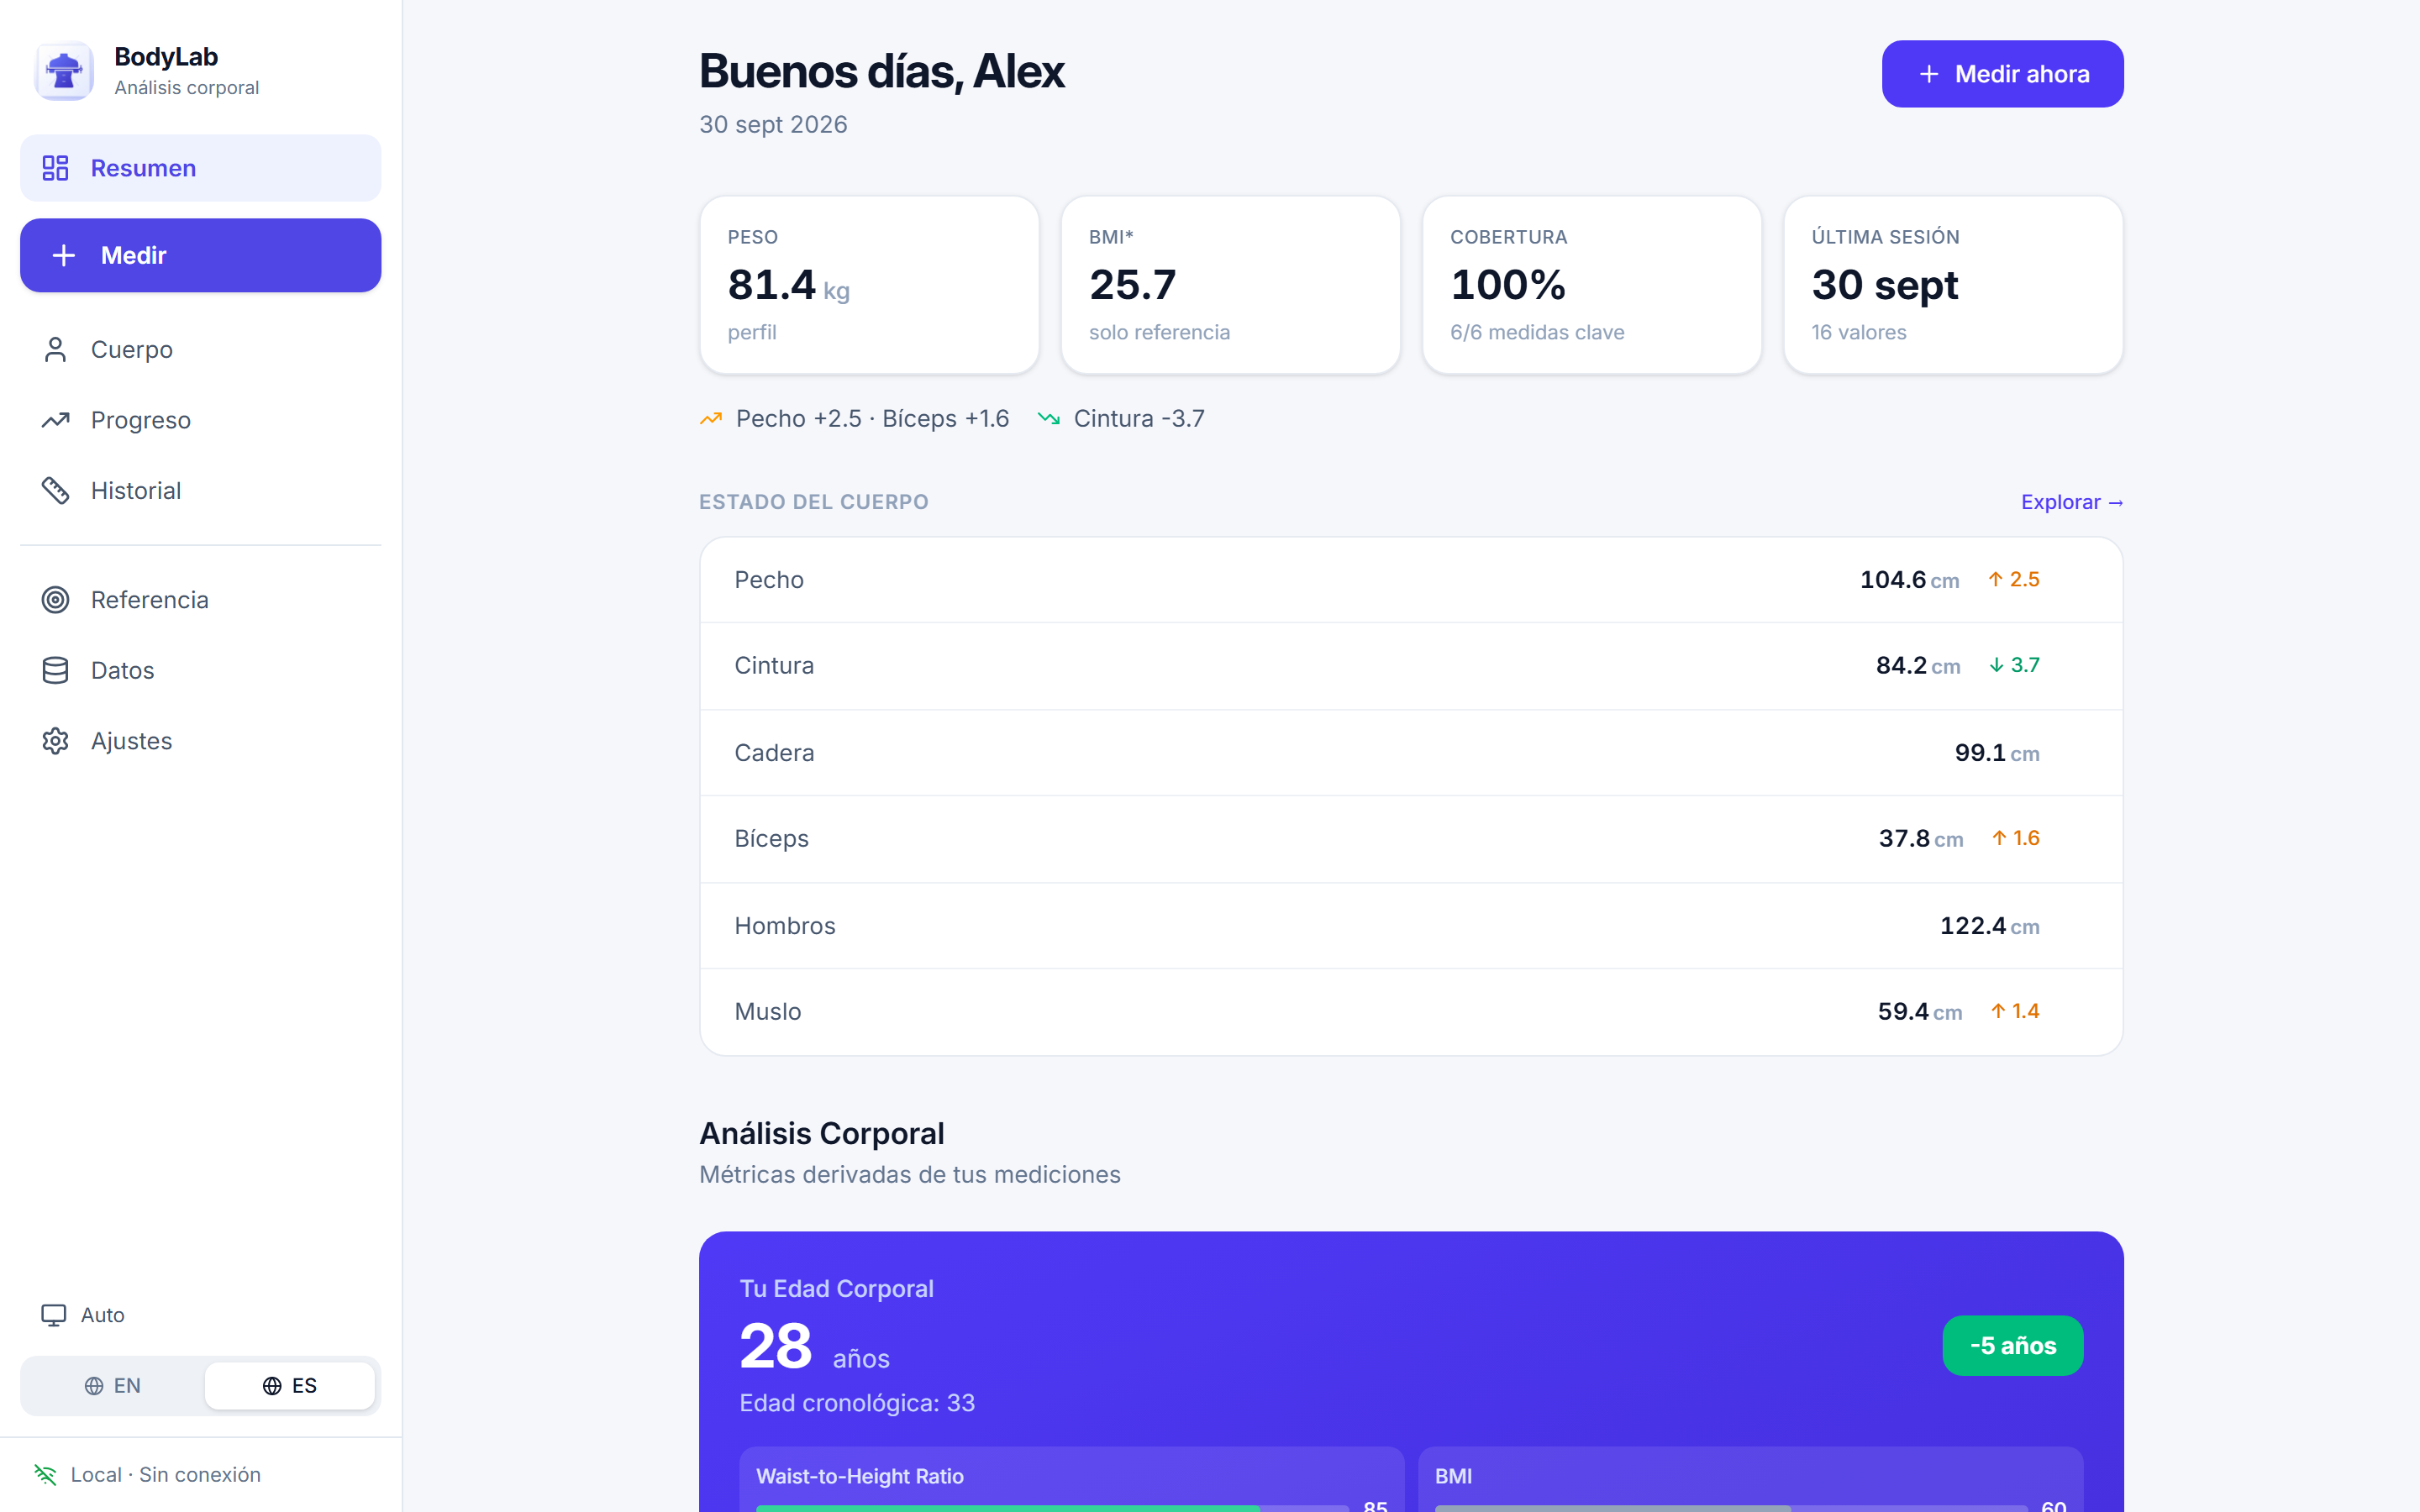
\includegraphics[width=\columnwidth]{../screenshots/bodylab-overview.png}
\caption{Panel principal: indicadores, anal\'itica y accesos a los flujos de
medici\'on.}
\label{fig:overview}
\end{figure}

\subsection{Medici\'on guiada (\code{/measure})}
594 l\'ineas de l\'ogica: es la pantalla m\'as densa del producto y la que
materializa la filosof\'ia. Presenta cada medici\'on con su instrucci\'on
t\'ecnica, agrupa los pasos en sesiones y muestra el progreso. El usuario puede
guardar la sesi\'on parcialmente; el historial nunca se sobrescribe, de modo que
un error de hoy es un dato de hoy y no la destrucci\'on de la medici\'on de ayer.

\subsection{Historial (\code{/history})}
1000 l\'ineas: la pantalla que m\'as creci\'o con el uso real
(Fig.~\ref{fig:history}). Presenta series por m\'etrica con el historial
completo y permite comparar dos momentos. Un defecto real detectado en
producci\'on justifica el modelo de verificaci\'on descrito en la
Sec.~VIII: la minificaci\'on convirti\'o una lectura antes de declaraci\'on
(\emph{temporal dead zone}) en una pantalla en blanco, invisible en desarrollo y
visible para el usuario. La correcci\'on se acompa\~n\'o de una prueba que monta
cada pantalla del producto.

\begin{figure}[t]
\centering
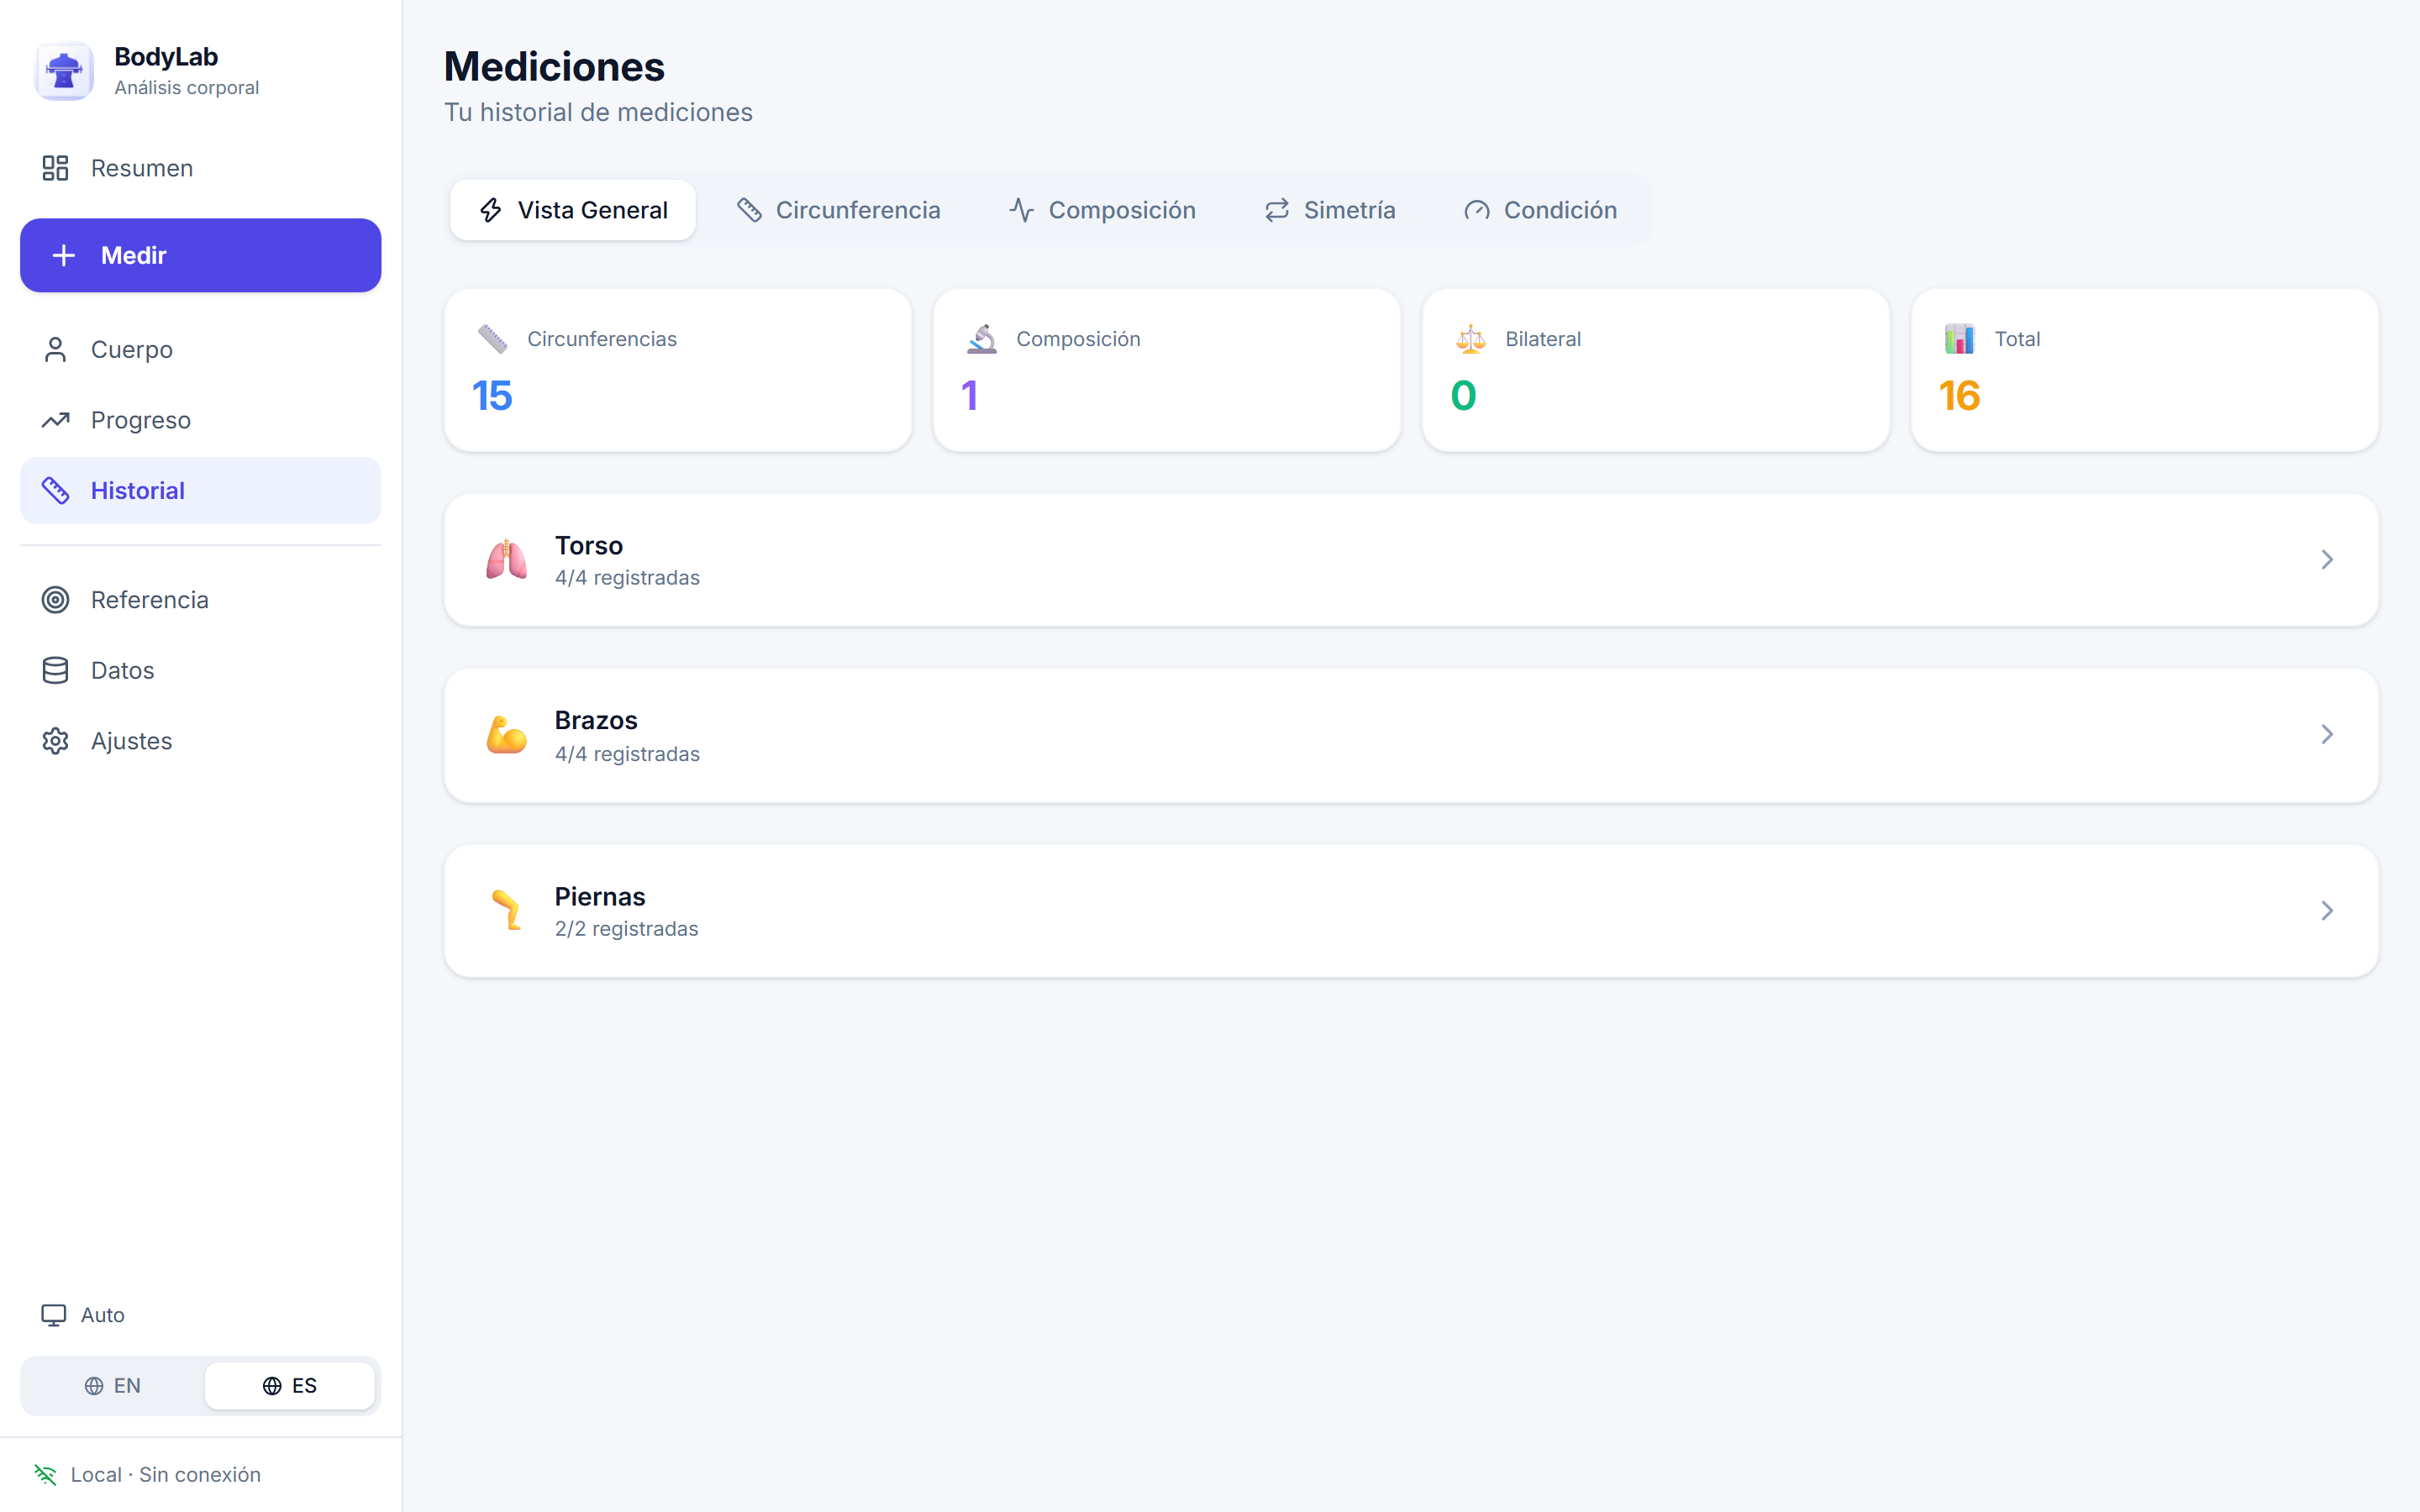
\includegraphics[width=\columnwidth]{../screenshots/bodylab-history.png}
\caption{Historial: series temporales con historial completo y comparaci\'on
entre instant\'aneas.}
\label{fig:history}
\end{figure}

\subsection{Cuerpo (\code{/body})}
Tres bloques en una columna: mapa muscular 2D interactivo, explorador 3D
importado de forma diferida y registro de ejercicio con gu\'ias animadas. La
pesta\~na 3D se carga s\'olo si el usuario la abre, y el registro de ejercicio
escribe en el mismo almac\'en que consume TrainingLab al exportar.

\subsection{Progreso (\code{/progress})}
Compara dos instant\'aneas cualesquiera lado a lado, con la l\'inea temporal
completa. Es la pantalla que responde ``¿estoy mejor que hace tres meses?'' sin
adjetivos.

\subsection{Referencias (\code{/references})}
Define y muestra los perfiles de referencia. Aqu\'i se hace expl\'icito el
compromiso del producto: la referencia es un par\'ametro del an\'alisis, no una
autoridad moral.

\subsection{B\'oveda de datos (\code{/data})}
Exportaci\'on e importaci\'on completa en formato \code{.bodylab}, m\'as CSV y
JSON. Es la \'unica pantalla que habla directamente con el adaptador de base de
datos, porque su unidad de trabajo es la base entera y no una entidad. La
existencia de esta pantalla es lo que hace cre\'ible la promesa
\emph{local-first}: los datos se pueden sacar.

\subsection{Preferencias (\code{/settings})}
Idioma, tema, unidades y opciones de privacidad. La actualizaci\'on de la
aplicaci\'on de escritorio vive aqu\'i y es \emph{manual}: se consulta cuando el
usuario lo pide y nunca descarga en segundo plano.

\subsection{Tel\'efono}
La misma interfaz con el contrato de la Tabla~\ref{tab:contract}. La
Fig.~\ref{fig:phone} documenta el comportamiento verificado en un iPhone
(414$\times$896~px): cero controles por debajo de 44\,px, ning\'un campo con
tipograf\'ia inferior a 16\,px y sin desbordamiento horizontal.

\begin{figure}[t]
\centering
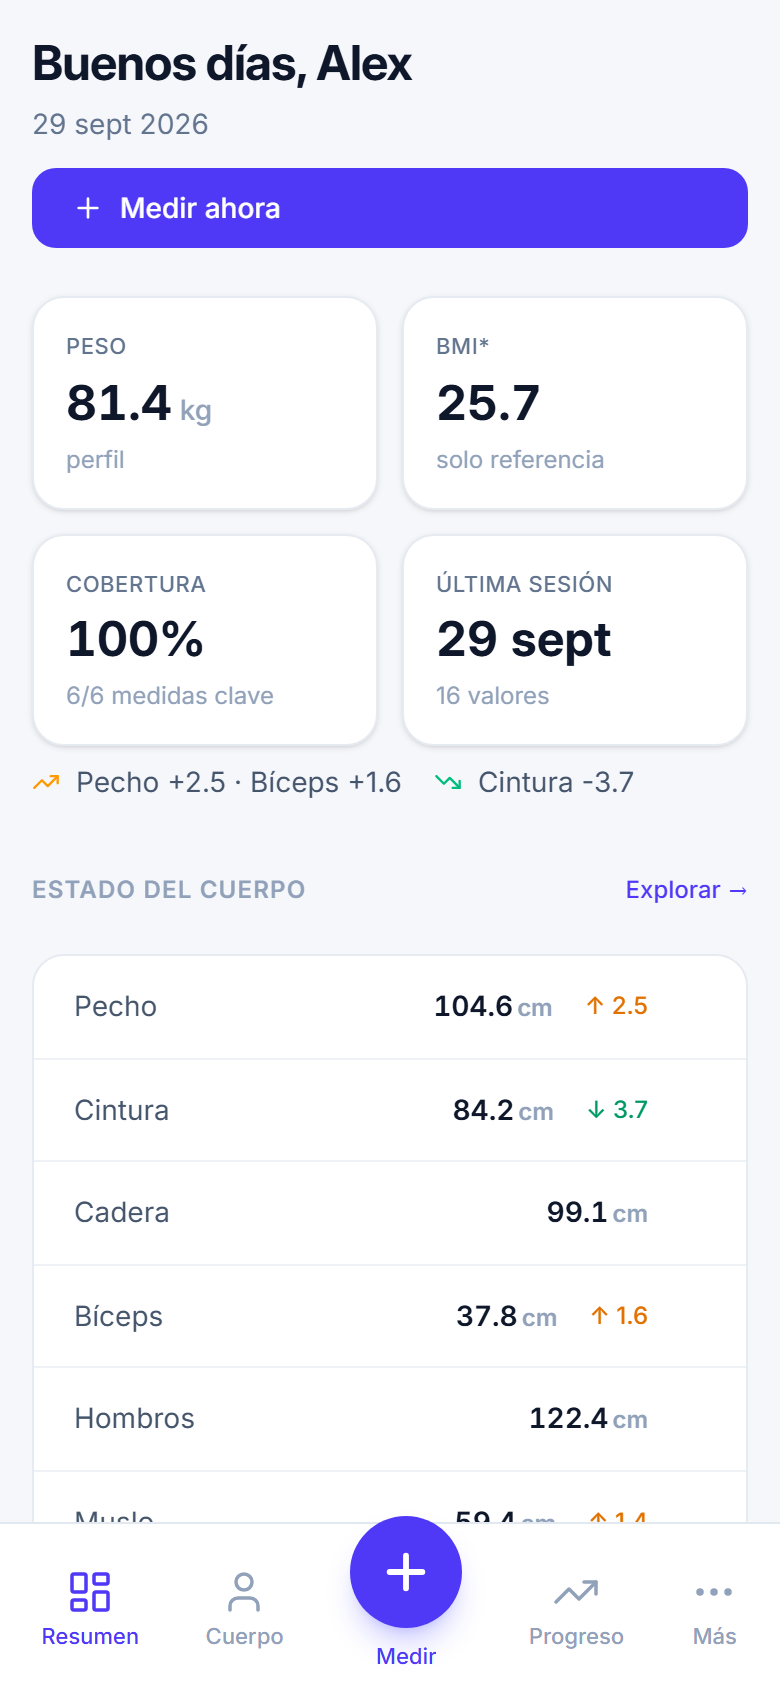
\includegraphics[width=0.72\columnwidth]{../screenshots/bodylab-phone.png}
\caption{Vista de tel\'efono: navegaci\'on inferior, objetivos t\'actiles y
respeto de las zonas seguras.}
\label{fig:phone}
\end{figure}

\section{Modelo de calidad}

La verificaci\'on es acumulativa y se ejecuta antes de cualquier publicaci\'on
(Tabla~\ref{tab:quality}).

\begin{table}[t]
\caption{Niveles de verificaci\'on}
\label{tab:quality}
\centering
\footnotesize
\begin{tabular}{@{}lrp{38mm}@{}}
\toprule
Nivel & N & Qu\'e protege \\
\midrule
N\'ucleo (ra\'iz) & 815 & f\'ormulas, contratos, base de datos, integridad de datos, adversarios \\
Interfaz (web) & 110 & p\'aginas, integraci\'on total, contratos con el n\'ucleo \\
Extremo a extremo & 21 & 14 flujos de producto, 5 de cero confianza, 2 de rayos X anat\'omicos \\
Est\'atico & --- & \code{oxlint} sin avisos, TypeScript estricto, Prettier \\
Invariantes & --- & auditor\'ia de cat\'alogo y de material \\
\bottomrule
\end{tabular}
\end{table}

Dos pr\'acticas merecen menci\'on. Primero, un umbral de cobertura del 80\,\% en
el n\'ucleo. Segundo, la documentaci\'on se verifica como el c\'odigo: las
capturas se generan con un gui\'on que siembra datos realistas en el paquete
compilado, exige una cadena esperada en pantalla y \emph{rechaza} la de estado
vac\'io. La primera versi\'on de ese gui\'on produjo cinco im\'agenes
id\'enticas del asistente de bienvenida; el fallo era del instrumento, no del
producto, y se corrigi\'o a\~nadiendo contexto de navegador por captura.

\section{Proceso de desarrollo y operaci\'on}

\subsection{Convenciones del c\'odigo}
El repositorio es un \emph{workspace} de pnpm sobre Node $\geq$ 20. Los
identificadores y comentarios van en ingl\'es; el texto visible de la interfaz va
en espa\~nol, con bienvenida biling\"ue gestionada por un diccionario central.
TypeScript es estricto en todo el \'arbol y la aplicaci\'on web a\~nade
\code{verbatimModuleSyntax} y \code{erasableSyntaxOnly}. El formato es
responsabilidad de Prettier y el an\'alisis est\'atico de \code{oxlint} (que se
exige sin avisos); no hay configuraci\'on de ESLint y a\~nadirla ser\'ia un
defecto de proceso.

Una convenci\'on merece ser destacada por su car\'acter de seguridad: \emph{nunca}
se interpreta una entrada num\'erica del usuario con \code{parseFloat} o
\code{parseInt} directos, porque el separador decimal espa\~nol (\code{75,5})
se truncar\'ia silenciosamente a 75. Existe un \'unico ayudante de parseo y es
obligatorio; la regla es de interfaz porque vive en los campos.

\subsection{Integraci\'on continua y distribuci\'on}
Los flujos de trabajo viven en la \textbf{ra\'iz} del repositorio, no dentro del
monorepositorio, porque el proveedor de integraci\'on continua no lee el
directorio de flujos de un subdirectorio; cada trabajo se ejecuta desde
\code{fitness-ecosystem} y las sobrescrituras de directorio por paso escriben la
ruta completa. Hay tres flujos: integraci\'on (pruebas, an\'alisis est\'atico,
tipos y compilaciones de producci\'on de ambas aplicaciones), publicaci\'on
(construye los instaladores de ambas aplicaciones, publica un \emph{alias}
estable para que los enlaces de descarga sobrevivan a los cambios de versi\'on, y
firma \'unicamente cuando existen los secretos) y despliegue de la demostraci\'on
p\'ublica. La disciplina de publicaci\'on es expl\'icita: \emph{se ejecuta la
puerta de verificaci\'on completa en local antes de subir nada, y se sube una sola
vez por bloque de trabajo}.

\subsection{Trazabilidad de requisitos}
La Tabla~\ref{tab:trace} relaciona cada compromiso del producto con su
implementaci\'on y con la verificaci\'on que lo protege.

\begin{table}[t]
\caption{Trazabilidad requisito $\rightarrow$ implementaci\'on $\rightarrow$ verificaci\'on}
\label{tab:trace}
\centering
\footnotesize
\begin{tabular}{@{}p{19mm}p{31mm}p{26mm}@{}}
\toprule
Requisito & Implementaci\'on & Verificaci\'on \\
\midrule
Sin servidor & IndexedDB y adaptador & pruebas de integridad de datos \\
Exportar todo & paquete \code{export} y b\'oveda & pruebas de exportaci\'on y flujos E2E \\
Funcionar sin red & aplicaci\'on est\'atica & sin peticiones de red \\
F\'ormulas citadas & \code{core/anthropometry} & 18 pruebas de referencias y composici\'on \\
N\'ucleo independiente & regla de revisi\'on & pruebas de contrato con el n\'ucleo \\
Licencias limpias & aviso de terceros y manifiesto & auditor\'ia de cat\'alogo y material \\
Contrato responsivo & capa de tokens y hoja de estilo & montaje de p\'aginas y auditor\'ia \\
\bottomrule
\end{tabular}
\end{table}

\section{Estado actual y hoja de ruta}

\subsection{Construido y verificado}
Motor antropom\'etrico y de composici\'on; cat\'alogo de 143 ejercicios con
rasgos, equipo, t\'ecnica y \emph{rig}; capa de material con licencias
documentadas; las ocho interfaces con contrato responsivo; aplicaci\'on de
escritorio con instalador firmable y actualizaci\'on manual; integraci\'on
diferida 3D; exportaci\'on completa; y el modelo de verificaci\'on descrito
arriba. N\'umero de referencia: 815 pruebas de n\'ucleo, 110 de interfaz y 21
flujos de navegador en verde.

\subsection{Estado objetivo}
El objetivo declarado no es a\~nadir funciones, sino cerrar tres frentes:
\begin{enumerate}
  \item \textbf{Cobertura did\'actica completa.} Cerrar los dos huecos que la
  auditor\'ia encontr\'o: trabajo de trapecio (hoy el vocabulario existe pero no
  hay ejercicios primarios suficientes) y un bloque de movilidad y
  \emph{stretching} que hoy es inexistente, con esquema de tiempo sostenido en
  lugar de series y repeticiones.
  \item \textbf{Material de las 43 entradas sin imagen.} Siluetas generadas
  localmente a partir del \emph{rig} propio (el rig produce mapas de postura en
  formato de puntos anat\'omicos que un modelo de difusi\'on local convierte en
  imagen), con revisi\'on humana obligatoria antes de publicar y sin usar nunca
  material de terceros como entrada.
  \item \textbf{Historial compartido del hogar.} Un registro opcional en la red
  local, con interruptor expl\'icito, para que varias personas de la casa
  compartan el mismo historial sin servidor externo ni cuenta.
\end{enumerate}

\subsection{Criterio de terminación}
El proyecto declara una versi\'on completa s\'olo si se cumplen
simult\'aneamente: 100\,\% de requisitos \code{MUST}, 100\,\% de los criterios
cr\'iticos de aceptaci\'on, 100\,\% de las pruebas cr\'iticas, cero defectos
prioridad~0 y~1, exportaci\'on y restauraci\'on correctas, funcionamiento sin
red, compilaci\'on de la versi\'on de escritorio, licencias y atribuciones
completas, documentaci\'on completa y alcance congelado. No se admite declarar
terminado ``porque se ve acabado''.

\section{Conclusiones}
BodyLab demuestra que una aplicaci\'on de medici\'on corporal puede ser
rigurosa, privada y comprensible a la vez: mantiene la matem\'atica en un
n\'ucleo puro y verificable, expone sus referencias, conserva el historial
completo y no pide permiso a ning\'un servidor para funcionar. El trabajo
pendiente no es de arquitectura sino de contenido y de cierre: completar la
cobertura did\'actica, dar imagen a las entradas que hoy s\'olo tienen dibujo, y
extender el historial al hogar sin romper la promesa de que los datos no salen
de la m\'aquina.

\begin{thebibliography}{9}
\bibitem{research} Proyecto Fitness. \emph{Validaci\'on de caracter\'isticas:
investigaci\'on de comunidades china y estadounidense}. Documento de
investigaci\'on del repositorio, 2026.
\bibitem{audit} Proyecto Fitness. \emph{Auditor\'ia de datos de ejercicios y
cobertura del cat\'alogo}. Documento de auditor\'ia del repositorio, 2026.
\bibitem{arch} Proyecto Fitness. \emph{Arquitectura de referencia del
monorepositorio}. Documento de arquitectura del repositorio, 2026.
\bibitem{spec} Proyecto Fitness. \emph{Especificaci\'on de producto y criterio
de terminaci\'on}. Documento de producto del repositorio, 2026.
\bibitem{ui} Proyecto Fitness. \emph{Contrato de dise\~no de interfaz y
reglas responsivas}. Documento de dise\~no del repositorio, 2026.
\end{thebibliography}

\end{document}
